\documentclass{school-22.101-notes}
\date{September 19, 2011}

\begin{document}
\maketitle

\lecture{Solve Time-Independent SEQ with 5 Potentials} \label{TISEQ}
Time-independent SEQ is important for two reasons:
\begin{enumerate}
\item We care about energy eigenvalue problem, which is time independent because energy conserves and thus do not change with respect to time. 
\item Solutions of time-independent SEQ are stationary states. For instance, \textbf{if $\ket{\psi} = \ket{E}$, then the system is stationary.}
\end{enumerate}
In this section, we will cover 3 unbounded systems (free particle, simple step barrier, rectangular barrier), and 2 bounded systems (infinite potential well, finite potential well). 

%%%%%%%%%%%%%%%%%% Overview %%%%%%%%%%%%%%%%%%%
\topic{Unbound vs. Bound States}
To solve the specific SEQ, we need to know the potential. In this class we have two types of potentials:
\begin{enumerate}
\item \hi{Unbound States: where $E > 0$.}
  \begin{enumerate}
  \item Scattering states, travelling of waves.  We define bound states to be the ones satisfying:
    \eqn{ |\psi|^2 \to 0, x \to \infty  \mbox{ or } \int_{-\infty}^{\infty} |\psi|^2 \dx < \infty}
  \item Continuous energy; all energies are solutions. 
  \item BC problem for the energy eigenvalue equation. 
  \item Common problems:
    \begin{itemize}
    \item Free Particle: Chapter~\ref{free-particle}.
    \item Simple Step Barrier: Chapter~\ref{simple-step-barrier}.
    \item Rectangular Barrier: Chapter~\ref{rectangular-barrier}.
    \end{itemize}
  \end{enumerate}

  \item \hi{Bound States: where $E<0$.}
    \begin{enumerate}
      \item System constrained in a region of space (e.g., bound particles as atoms/nuclei, commonly found in nuclear structures). 
      \item Quantization of energy (energy levels).
      \item BC problem for $E_n$ eigenvalue equation. 
      \item Common problems: 
        \begin{itemize}
        \item Infinite square well with $E<0$, see Chapter~\ref{infinite-square-well}. 
        \item Finite square well with $E<0$. We first solve it in Chapter~\ref{finite-square-well}, then solve it in the context of deuteron in Chapter~\ref{2H-bound-state} by adding in $l$ and $s$.
        \end{itemize}
        Notice we specify $E<0$, because we can have a finite square well, but if the particles have $E>0$, then the particles can travel everywhere as a free particle, making it a unbound state. 
    \end{enumerate}
\end{enumerate}

%%%%%%%%%%%%%%% Free Particle %%%%%%%%%%%%%%%
\topic{Free Particle, Concept of Flux\label{free-particle}}
Recall we solved already 1D free particle problem and found, 
\begin{itemize}
\item $\hat{H} = \hat{K} = \frac{\hat{p}^2}{2m} = - \frac{\hbar^2}{2m} \laplacian$. 

\item The energy eigenvalue problem is, 
  \eqn{ - \frac{\hbar^2}{2m} \ppsipxn2 &= E \psi(x) }
  and the energy eigenvalue is, 
  \eqn{ E = \frac{\hbar^2 k^2}{2m} }

\item Stationary states are, 
  \eqn{ \psi(x) = A \sin(kx) + B \cos (kx) }
  Travelling waves are, 
  \eqn{ \psi(x) = A e^{ikx} + B e^{-ikx} }

\item The probability of finding the particle is related to the square modular of the state function:
\eqn{ \mbox{Probability} = P(x \to x+\Delta x) \dx = |\psi(x)|^2 \dx   }
In the case of 1D free particle, $|A|^2 \dx$ is unitless, then $|A|^2$ is in the unit of 1/m. This unit gives us a hint that $|A|^2$ has to do with the `particle density' injected into the system, similar to $P(x\to x+\dx)$. Nextwe will relate it to flux. 

\item Typically $A$ is found by normalization $\int |\psi(x)|^2 \dx = 1$. But in the case of a travelling wave, as hinted above, $A$ should be found in terms of flux of particles. We know the `particle density', quantified as the `flux' , of the incoming beam of particles and assume it to be a constant. 
\eqn{ \mbox{Measured Flux } \Gamma = P(x) v= \frac{\hbar k}{m} |\psi (x)|^2 \mbox{ because } P(x) = |\psi(x)|^2, v = \frac{p}{m} = \frac{\hbar k}{m} }
Notice that the measured flux $\Gamma$ has a unit of 1/sec in 1D. In 3D the unit of flux would be particles/second per unit area. 

In the case of 1D scattering, we know $|\psi(x)|^2 = |A|^2$, then knowing the flux or particle density, we can find A from:
\eqn{ |A| = \sqrt{ \frac{\Gamma m}{\hbar k}  } }
Summary, knowing the incoming particles' $\Gamma$, we can find the energy of the incoming beams $E = \frac{\hbar^2 k^2}{2m}$, and we also know V(x) which is a potential barrier.

\item We take the state to be $\psi = A e^{ikx}$. Expand it to 3D (assuming time-independent for now):
\eqn{ u(\uline{r} ,t) = e^{i (\uline{k} \cdot \uline{r} - wt )} = e^{i \uline{k} \cdot \uline{r} }  = e^{\frac{i}{\hbar} \uline{p} \cdot \uline{r} } }
in which we used the relation $\uline{p} = \hbar \uline{k}$. Then we consider the angle between $\uline{p}, \uline{r}$ to be angle $\theta$, that is, 
\eqn{ \theta = \arccos\left( \frac{\uline{k} \cdot \uline{r}}{|\uline{k}| |\uline{r}|}    \right) }
Then in a simplified 1D case, $\theta$ can only take either 0 (in which case k is the same direction as r) or 1 (in which case k is the opposite direction of r). So our original $\psi = A e^{ikx}$ expression is actually two possibilities, either $+x, k>0$ or $-x, k<0$, whichever way when we multiply them, the product comes out to be positive. 
\end{itemize}




%%%%%%%%%%%%%%%%
\topic{Simple Step Barrier} \label{simple-step-barrier}
Set-up: Case A has an incoming KE of $E_A > V_H$. Case B has an incoming KE of $E_B < V_H$. Classically, we can predict that in case A the particle will continue travelling in region II, but with a reduced KE of $E_A - V_H$. In Case B, the particle will simply be reflected back with $E_B$. 

\subtopic{Case A: $E > V$}
\begin{figure}[h!]
    \centering
    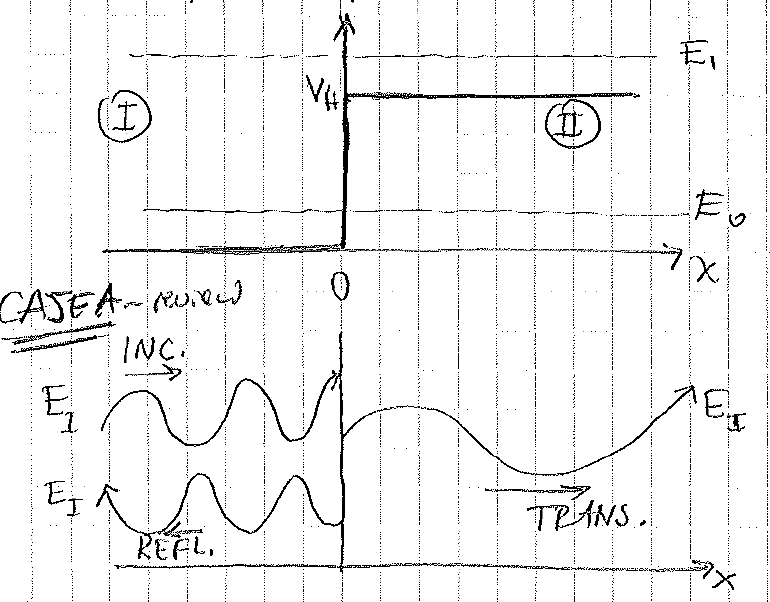
\includegraphics[width=4in]{images/qm/step-barrier-caseA.png}
    \caption{Simple Step Barrier Diagram, E$>$V}
\end{figure}

\begin{itemize}
\item Quantum mechanically, the wave would transmit and/or reflect upon hitting a step barrier. Intuitively, in this case we would get $E_{\mathrm{reflected}} = E_{\mathrm{incoming}}$ (thus reflecting with the same wavelength), as well as a transmitted wave with $E_{\mathrm{trans}} < E_{\mathrm{incoming}}$ (thus transmitted wave with wavelength larger than the incoming one). 

\item Region I: 
\eqn{ -\frac{\hbar^2}{2m} \ppsipxn2 = E_1 \psi, E_1 = \frac{\hbar^2 k_1^2}{2m} }
\eqn{ \ppsipxn2 + k_I^2 \psi = 0 \Rightarrow \psi_I = A e^{ik_1x} + B e^{-ikx_1x}  }

\item Region II:
\eqn{ -\frac{\hbar^2}{2m} \ppsipxn2 + V_H \psi = E_1 \psi  }
\eqn{ \ppsipxn2 + k_2^2 \psi = 0 \Rightarrow \psi_{II} = C e^{ik_2 x} + D e^{-ik_2 x} }
in which $k_2^2 = \frac{2m (E_1 - V_H)}{\hbar^2}$, or $E_1  = \frac{\hbar^2 k_2^2}{2m} + V_H$. Notice in Region II, there is no source of neutrons that wolud travel to the left, thus only the C term survives. 
\eqn{ \psi_{II} = C e^{ik_2 x} }

\item BC1: $\psi(0^-) = \psi(0^+)$, thus $A+B = C$. 

\item BC2: $\left. \dpsidx \right|_{x=0^-} = \left. \dpsidx \right|_{x=0^+}$, thus $(A - B) k_1 = C k_2$. 

Together we can write $B, C$ in terms of $A$:
\eqn{ B = \frac{k_1 - k_2}{k_1 + k_2} A, \fsp C = \frac{2 k_1}{k_1 + k_2} A }

\item Prove conservation of flux. Mathematically we can write 
\eqn{ \frac{\hbar k_1}{m} |A|^2 = \frac{\hbar k_1}{m} |B|^2 + \frac{\hbar k_2}{m} |C|^2 }
This leads us to define \hi{flux} which is $\Gamma = \mathrm{Prob} v = |C_n|^2 \frac{\hbar k}{m}$: 
\eqn{ \Rightarrow k_1 |A|^2 = k_1 |B|^2 + k_2 |C|^2 }
\eqn{ \Rightarrow \Gamma_{\mbox{INC}} = \Gamma_{\mbox{REFL}} + \Gamma_{\mbox{TRANS}}  }
\eqn{ \Rightarrow 1 = \frac{\Gamma_{\mbox{REFL}}}{\Gamma_{\mbox{INC}}} + \frac{\Gamma_{\mbox{TRANS}}}{\Gamma_{\mbox{INC}}}  =  T + R }
where T is the transition probability/coefficient, and R is the reflection probability/coefficient:
\eqn{ R = \frac{|B|^2}{|A|^2}, \fsp T = \frac{k_2 |C|^2}{k_1 |A|^2} } 

\item Case A recap: 
$\psi_1 (x) = A e^{ik_1 x} + B e^{i k_2 x}$ in which $k_1 = \sqrt{\frac{2 m E_1}{\hbar^2}}$. \\
$\psi_2 (x) = C e^{ik_2 x}$ in which $k_2 = \sqrt{\frac{2 m (E_1 - V_H)}{\hbar^2}}$. 

Apply BC, we can find the relationship between A,B,C. 

Apply conservation of flux $\Gamma_{\mbox{INC}} = \Gamma_{\mbox{REFL}} + \Gamma_{\mbox{TRANS}}$, and given $\Gamma = P(x) v$ in which $P(x) = |\psi|^2, v = \frac{\hbar k}{m}$, we know: 
\eqn{ \frac{\hbar k_1}{m} |A|^2 = \frac{\hbar k_1}{m} |B|^2 + \frac{\hbar k_2}{m} |C|^2 }
in which R and T are defined as:
\eqn{ R = \frac{|B|^2}{|A|^2}, \fsp T = \frac{k_2 |C|^2}{k_1 |A|^2} } 
\end{itemize}



\subtopic{Case B: $E < V$}
\begin{figure}[h!]
    \centering
    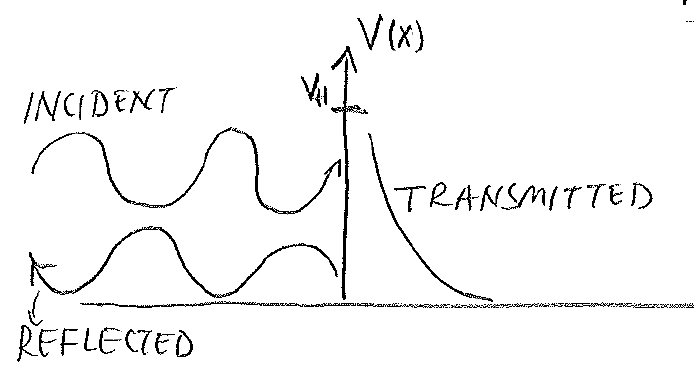
\includegraphics[width=4in]{images/qm/step-barrier-caseB.png}
    \caption{Simple Step Barrier Diagram, E$<$V}
\end{figure}

\begin{itemize}
\item Region I: 
\eqn{ \psi_1 (x) &= A e^{ik_1 x} + B e^{i k_2 x}  & k_1 &= \sqrt{\frac{2 m E_1}{\hbar^2}} }

\item Region II:
\eqn{ \psi_2 (x) &= C e^{ik_2 x}  & k_2 &= \sqrt{\frac{2 m (E_1 - V_H)}{\hbar^2}}}
Notice now that $E_1 - V_H < 0$, $k_2^2$ is going to be negative. We define $\kappa^2 = - k_2^2 = \frac{2 m (V_H - E_1)}{\hbar^2}$, then $k_2 = \mp i \kappa$.
\eqn{ \psi_2 (x) = C e^{-\kappa x} + D e^{ \kappa x} }
We know for $x \to \infty, \psi_2 \neq \infty, \Rightarrow D = 0$. 
\eqn{ \psi_2 (x) = C e^{-\kappa x} }

\item Apply BC, we can find the relationship between A,B,C:
\eqn{ \psi_1 (0) = \psi_2 (0) \Rightarrow A + B = C }
\eqn{ \psi_1^{\prime} (0) = \psi_2^{\prime} (0) \Rightarrow i k_1 (A-B) = - \kappa C }

That is to say,
\eqn{ B = \frac{k_1 - i \kappa}{k_1 + i \kappa} A, \fsp C = \frac{2 k_1}{k_1 + i \kappa} A }

\item The expression we get for B,C as a function of A is simlar to last time, so our conservation of flux relation holds true. Then we can write: 

\eqn{ \frac{|B|}{|A|} = \frac{|k_1 - i \kappa|}{|k_1 + i \kappa|} = \frac{|z^*|}{|z|} }
\eqn{ \frac{|B|^2}{|A|^2} = \frac{(k - i\kappa)(k+ i \kappa) } {(k+ i\kappa) (k - i \kappa)} = 1 \Rightarrow R = \frac{|B|^2}{|A|^2} = 1 }

\item Interpretation: $R = 1$ means \uline{all the particles would EVENTUALLY be reflected back.} But $T \neq 0$ means at certain part of region 2, we might find particles (this can also be seen from the fact that $\psi_2 = C e^{-\kappa x}, P(x) = |C|^2 e^{-2 \kappa x}$). \textbf{These particles are going through a finite penetration before it is entually reflected back.} During the region of finite penetration in region 2, the beam's probability decay exponentially in the form of $e^{-2\kappa x}$. 

The smaller $\kappa$ is (hence the larger E is), the more the particle would penetrate the material. 
\end{itemize}

\end{document}
